\documentclass[a4paper,12pt]{article}

%%% Работа с русским языком
\usepackage{cmap}					% поиск в PDF
\usepackage{mathtext} 				% русские буквы в формулах
\usepackage[T2A]{fontenc}			% кодировка
\usepackage[utf8]{inputenc}			% кодировка исходного текста
\usepackage[english,russian]{babel}	% локализация и переносы
\usepackage{indentfirst}
\frenchspacing


%%% Дополнительная работа с математикой
\usepackage{amsmath,amsfonts,amssymb,amsthm,mathtools} % AMS
\usepackage{icomma} % "Умная" запятая: $0,2$ --- число, $0, 2$ --- перечисление

%% Номера формул
%\mathtoolsset{showonlyrefs=true} % Показывать номера только у тех формул, на которые есть \eqref{} в тексте.
%\usepackage{leqno} % Нумерация формул слева

%% Свои команды
\DeclareMathOperator{\sgn}{\mathop{sgn}}

%% Перенос знаков в формулах (по Львовскому)
\newcommand*{\hm}[1]{#1\nobreak\discretionary{}
	{\hbox{$\mathsurround=0pt #1$}}{}}

%%% Работа с картинками
\usepackage{graphicx}  % Для вставки рисунков
\graphicspath{{images/}}  % папки с картинками
\setlength\fboxsep{3pt} % Отступ рамки \fbox{} от рисунка
\setlength\fboxrule{1pt} % Толщина линий рамки \fbox{}
\usepackage{wrapfig} % Обтекание рисунков текстом

%%% Работа с таблицами
\usepackage{array,tabularx,tabulary,booktabs} % Дополнительная работа с таблицами
\usepackage{longtable}  % Длинные таблицы
\usepackage{multirow} % Слияние строк в таблице

%%% Теоремы
\theoremstyle{plain} % Это стиль по умолчанию, его можно не переопределять.
\newtheorem{theorem}{Теорема}[section]
\newtheorem{proposition}[theorem]{Утверждение}

\theoremstyle{definition} % "Определение"
\newtheorem{corollary}{Следствие}[theorem]
\newtheorem{problem}{Задача}[section]

\theoremstyle{remark} % "Примечание"
\newtheorem*{nonum}{Решение}

%%% Программирование
\usepackage{etoolbox} % логические операторы

%%% Страница
\usepackage{extsizes} % Возможность сделать 14-й шрифт
\usepackage{geometry} % Простой способ задавать поля
\geometry{top=15mm}
\geometry{bottom=20mm}
\geometry{left=20mm}
\geometry{right=20mm}
%
%\usepackage{fancyhdr} % Колонтитулы
% 	\pagestyle{fancy}
%\renewcommand{\headrulewidth}{0pt}  % Толщина линейки, отчеркивающей верхний колонтитул
% 	\lfoot{Нижний левый}
% 	\rfoot{Нижний правый}
% 	\rhead{Верхний правый}
% 	\chead{Верхний в центре}
% 	\lhead{Верхний левый}
%	\cfoot{Нижний в центре} % По умолчанию здесь номер страницы

\usepackage{setspace} % Интерлиньяж
%\onehalfspacing % Интерлиньяж 1.5
%\doublespacing % Интерлиньяж 2
%\singlespacing % Интерлиньяж 1

\usepackage{lastpage} % Узнать, сколько всего страниц в документе.

\usepackage{soul} % Модификаторы начертания

\usepackage{hyperref}
\usepackage[usenames,dvipsnames,svgnames,table,rgb]{xcolor}
\hypersetup{				% Гиперссылки
	unicode=true,           % русские буквы в раздела PDF
	pdftitle={Заголовок},   % Заголовок
	pdfauthor={Автор},      % Автор
	pdfsubject={Тема},      % Тема
	pdfcreator={Создатель}, % Создатель
	pdfproducer={Производитель}, % Производитель
	pdfkeywords={keyword1} {key2} {key3}, % Ключевые слова
	colorlinks=true,       	% false: ссылки в рамках; true: цветные ссылки
	linkcolor=violet,          % внутренние ссылки
	citecolor=black,        % на библиографию
	filecolor=orange,      % на файлы
	urlcolor= blue           % на URL
}

\usepackage{csquotes} % Еще инструменты для ссылок

%\usepackage[style=authoryear,maxcitenames=2,backend=biber,sorting=nty]{biblatex}

\usepackage{multicol} % Несколько колонок

\usepackage{tikz} % Работа с графикой
\usepackage{pgfplots}
\usepackage{pgfplotstable}

\renewcommand{\phi}{\varphi}
\renewcommand{\epsilon}{\varepsilon}
\usepackage[backend=biber]{biblatex}

\addbibresource{Semkin_2023_Lockdown.bib}

\title{Investigation of graph SIR+ model and lockdown's restrictions effects}
\author{Сёмкин К. \and Бишук А.}
\date{}

\begin{document}
	
	\maketitle
	
	\begin{abstract}
		Задача создания и обоснования математических моделей распространения эпидемий всегда являлась и будет являться актуальной в наше время. Существуют оправданные и реалистичные модели распространения, такие как SIR и SIER, основанные на дифференциальных уравнениях динамики количества больных и здоровых жителей, но их область применимости ограничивается большими масштабами наблюдения. В данной работе рассматривается аналог SIR, основанный на графе контактов, для анализа заболеваемости на малых мастштабах (предприятие, небольшая коммуна), исследуется вероятностная динамика распространения эпидемии в зависимости от параметров модели, а также влияние разных ограничительных мер. В частности интересно обоснование противоречивого эффекта, связанного с ростом заболевших при введении локдауна. Все теоретичские результаты демонстрируются проведением численных экспериментов посредством сэмплирования эпидемии на графе контактов, а также на основе реальных данных.
	\end{abstract}
	
	\section*{Introduction}
	
	В связи с известными событиями интерес к эпидемиологии и её методам сильно вырос. Для понимания динамики протекания короновирусной инфекции в 2020 году в разных местах Земли и на разных масштабах, а также для подготовки к будущим вспышкам заболеваемости, как никогда актуально построение адекватных математических моделей развития болезней в людских популяциях. Классические техники моделирования эпидемий опираются на параметризованные автономные системы дифференциальных уравнений, описывающие динамику изменения количества болеющих и здоровых людей. Эти модели дают хорошее понимание протекания болезни на больших масштабах (города, страны), но не способны описывать заболевание в небольших общественных структурах, например, промышленное предприятие, небольшую деревню или студенческое общежитие. В данной работе исследуется графовый подход к моделированию распространения инфекции, а именно вводится \textit{граф контактов}, по которому болезнь может <<кочевать>>. В качестве представления болезни используется стандартная для эпидемиологии модель SIR/SEIR, в которой каждому человеку (вершине в графе) сопоставляется некоторое состояние (больной, здоровый и т.д.), после чего в дискретном времени происходят смены этих состояний с некоторыми вероятностями и система эволюционирует.
	
	Также исследуются различные эффекты от мер по борьбе с инфекцией, таких как тестирование, изоляция и, самое интересное, \textit{локдаун}. Именно ему уделяется основное внимание, так как его введение может привести к необычному последствию --- росту заболеваемости среди населения. Но обнаружить такое поведение в стандартных моделях не представляется возможным, поэтому цель данной работы --- найти условия возникновения такого эффекта в модели и продемонстрировать его на численных экспериментах. 
	
	Изучение эпидемий на больших популяциях позволяет моделировать этот процесс в среднем, и даже получать точные аналитические решения \cite{harko2014exact}. В зависимости от поставленной прикладной задачи возникает необходимость моделировать процесс эпидемии с разной степенью подробности. Так, например, простейшая модель SI \cite{allen1994some} рассматривает всего два состояния: больной и здоровый. В этой модели не рассматривается формирование иммунитета: здоровый всегда может заразиться при контакте с инфекцией. Существуют модели, рассматривающие дополнительно формирование иммунитета, инкубационный период, летальные исходы и многие другие возможные состояния. Одной из таких моделей является SEIR(S) \cite{capasso2008mathematical}. Моделирование в среднем не подходит для небольших или слишком разнородных популяций. Эту проблему позволяют решить модели распространения эпидемии на графах \cite{moreno2002epidemic}, \cite{pastor2015epidemic}. Распространение эпидемии на графе контактов можно рассматривать, например, при помощи цепи Маркова \cite{gomez2010discrete}. Однако моделирование распространения болезни на больших графах со сложной структурой имеет высокую алгоритмическую сложность. Наиболее распространенной является задача прогнозирования течения эпидемии \cite{leitch2019toward} и оценка индивидуальных рисков. Результаты изучения распространения эпидемии на графах	могут быть использованы не только для анализа заболеваний. Например, распространение слухов или автомобильного трафика можно описать схожим математическим аппаратом \cite{de2013anatomy}. Базой для данной статьи является \cite{base_article}, где, в частности, введена модель болезни на графе и где в её рамках исследован эффект локдауна.
	
	В работе ставится задача обобщить модель из \cite{base_article}, сформулировать новые условия возникновения роста заболеваемости при введении карантина и явно показать этот эффект в численном эксперименте. Т.о. появится возможность испытывать обновлённую модель в более широком спектре реальных ситуаций, а также пересмотреть локдаун как однозначно позитивную меру противодействия эпидемии.
	
	\section*{Problem statement}
	
	Формально задача состоит в выявлении зависимости роста заболеваемости при введении локдауна от графа контактов и параметров динамики развития болезни.
	
	Пусть $ G = (V, E) $ --- исходный граф контактов, $ G^q = (V^q, E^q) $ --- граф контактов при введении карантинного режима. Ребро этих графов соответствует контакту данных лиц, а вес ребра $ \beta_{ij} $ соответствует вероятности вершины заразиться, если её сосед сам находится в состоянии \textit{Infected (I)}. 
	
	Будем понимать под $ G_t $ граф контактов на дискретном временном шаге $ t $, т.е. его графовую структуру, а также состояния каждой вершины в данный момент. Под $ I(G) $ будем понимать множество больных вершин в графе (или кол-во больных в графе, в зависимости от контекста). 
	
	Т.о. задача состоит в поиске условий на $ t_0 $, $ G $ и $ G_q $, при которых $ \underset{t \ge t_0}{\max} \, I(G^q_t) \ge \underset{t \ge t_0}{\max} \, I(G_t) $, где $ t_0 $ момент введения локдауна. Другая возможная постановка: найти условия на те же параметры, при которых $ \beta_{ij}^q \ge \beta_{ij} $.
	
	\section{Computational experiment}
	
	Главная задача вычислительного эксперимента --- проиллюстрировать эффект локдауна, сэмулировав эпидемию на графах контактов, в которых такой эффект вообще возможен. Т.о. данная демонстрация служит подтверждением неголословности оговоренного ранее.
	
	\subsection*{Basic algorith}
	
	Для начала были проведены симулирования заболеваемости с помощью библиотеки SEIRSplus \cite{seirsplus}, которая предоставляет богатые средства инициализации модели, а также её тонкой настройки в любой момент развития эпидемии. Стандартный граф контактов генерировался на заданном наборе вершин $ V = \{1, \ldots, N\} $ и содержал случайное количество рёбер, которое было точно больше половины числа ребёр в полносвязном графе. Граф карантина же собирался из клик случайного размера от 1 до 5 вершин. Чувствительность к заболеванию генерировалась случайно для каждой вершины, со средним вокруг значения $ 0.5 $, вероятность восстановления у заболевших вершин была одна для всех $ 0.3 $. 
	
	В итоге запускалось две симуляции, в одной из которых карантин не вводился, а в другой вводился на некоторое время. Результаты приведены на рис. \ref{pic:basic}. Здесь представлена динамика количества заражённых узлов для размера популяции $ 10, 100, 500 $ вершин в графе. Синия линия --- развитие болезни без локдауна, красная и розовая --- развитие с локдауном, где розовая линия как раз отвечает периоду изоляции. Зелёными линиями обозначены точки входа и выхода из локдауна.
	
	К сожалению, данная библиотека хоть и обладает огромным потенциалом, но всё же является технически недоработанной, а также скрывает в себе некоторые нежелательные методы ускорения сэмплирования, что не является приемлемым для текущего исследования. 
	
	\begin{figure}[h]
		\begin{minipage}{0.49\linewidth}
			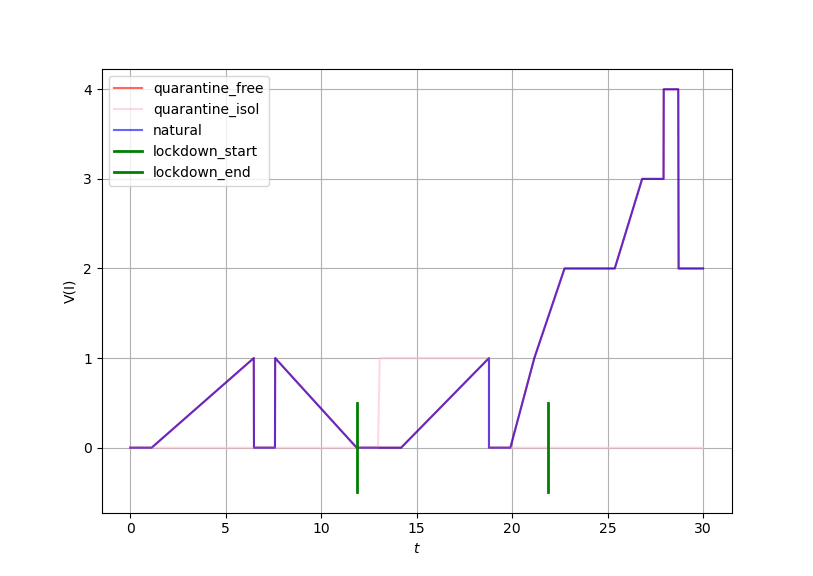
\includegraphics[width=\linewidth, keepaspectratio]{../figs/basic_experiment_small_population}
			
			\centering
			Small population
		\end{minipage}
		\begin{minipage}{0.49\linewidth}
			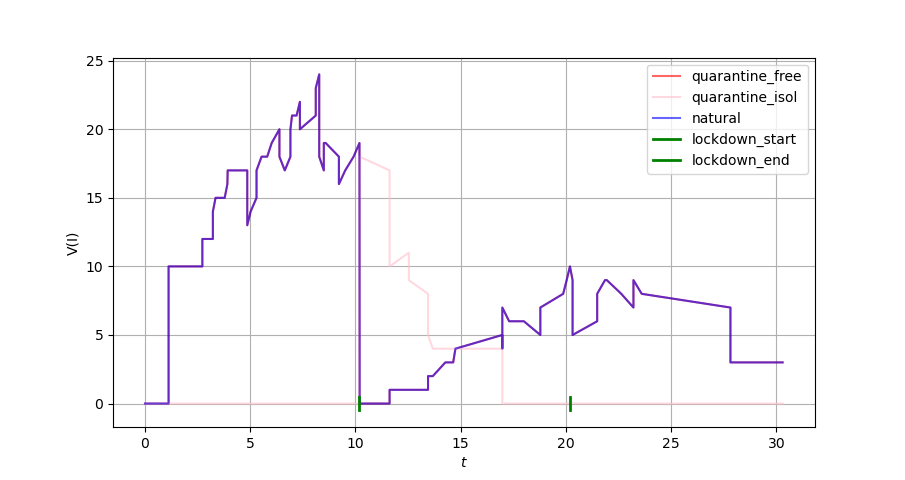
\includegraphics[width=\linewidth, keepaspectratio]{../figs/basic_experiment_medium_population}
			
			\centering
			Medium population
		\end{minipage}
		\begin{center}
			\begin{minipage}{0.5\linewidth}
			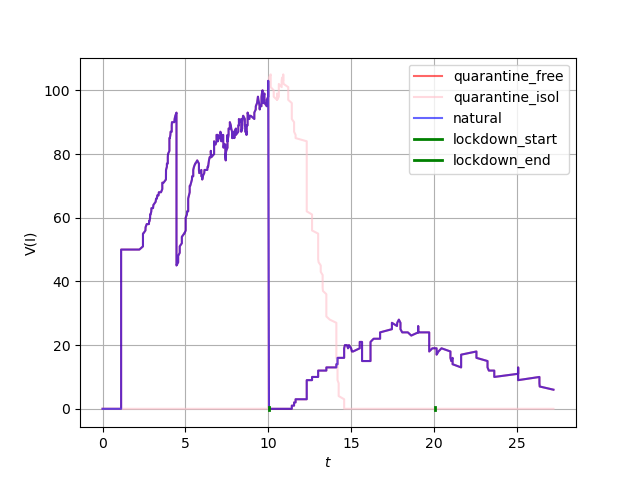
\includegraphics[width=\linewidth, keepaspectratio]{../figs/basic_experiment_big_population}
			
			\centering
			Large population
		\end{minipage}
		\end{center}
		\caption{Графики количества заражённых в двух режимах протекания эпидемии от времени}\label{pic:basic}
	\end{figure}

	\subsection*{Main experiment}
	
	
	
	\printbibliography
	
\end{document}